\chapter{Implementáció}

\section{Theta keretrendszer}
\label{sec:theta_keretrendszer}

A \emph{Theta}\footnote{\url{https://github.com/FTSRG/theta}} egy nyílt forráskódú, általános célú, moduláris és konfigurálható modellellenőrző keretrendszer, melyet absztrakciós finomításon alapuló algoritmusok tervezésének és értékelésének támogatására hoztak létre a különböző formalizmusok elérhetőségi elemzéséhez.

A keretrendszer a már évek óta tartó fejlesztéseknek köszönhetően számos eszközt tud nyújtani modellellenőrzéshez:\footnote{2020 decemberének elején.}

\begin{itemize}
	\item \verb+theta-cfa-cli+ -- Control Flow Automata hibahelyeinek\footnote{Az angol irodalom a \emph{location} kifejezést használja. Én a dolgozatomban a magyar megfelelőjét használom. TODO: nincs ez előbb definiálva már?} elérhetőségét vizsgálja CEGAR alapú algoritmusokkal
	
	\item \verb+theta-sts-cli+ -- \emph{Symbolic Transition Systems} biztonsági tulajdonságainak verifikációját végzi CEGAR alapú algoritmusokkal
	
	\item \verb+theta-xta-cli+ -- Uppaal időzített automaták verifikációját lehet vele elvégezni
	
	\item \verb+theta-xsts-cli+ -- \emph{eXtended Symbolic Transition Systems} biztonsági tulajdonságainak verifikációját végzi CEGAR alapú algoritmusokkal
\end{itemize}
\ \\
A Theta architektúrája négy rétegre osztható. Nevezetesen:

\begin{itemize}
	\item \textbf{Formalizmusok} -- A Theta legalapvetőbb elemei, melyek való-életbeli problémákat modelleznek le (pl. szoftvereket, hardvereket, protokollokat). A formalizmusok általában alacsony szintű, matematikai ábrázolások melyek elsőrendű logikai kifejezéseken és gráfszerű struktúrákon alapulnak. Ilyen például a \emph{Control Flow Automata}.
	
	\item \textbf{Háttéranalízis} -- Itt történik a formalizmus feldolgozása és ellenőrzése. Ide sorolható a program melyet fejlesztettem.
	
	\item \textbf{Sat-megoldó interfész} -- Ennek segítségével történik a verifikáció. A Theta a Z3 Sat-megoldót használja jelenleg.
	
	\item \textbf{Eszközök} -- Parancssori alkalmazások melyek futtatható \verb+jar+ fájlba fordíthatóak le. Jellemzően csak beolvassák az inputot és meghívják az alsóbb szinten lévő algoritmusokat. TODO: tud az enyém parancssorból futni?
	
\end{itemize}

\section{A program implementálása}

\subsection{Bemenet}
A program bemenete egy CFA, mely számos hellyel rendelkezik, melyek közül kiemelkedik a kezdő-, a hiba- illetve a végső hely. Az utóbbit a k-indukciós algoritmus nem veszi figyelembe, mert az a teljes teret bejárja, viszont más algoritmusok működéséhez szükségesek lehetnek. Az ezután következő \ref{sec:kiertekeles}. fejezetben részletesen kitérek a programom tesztelésére, de elöljáróban azt érdemes tudni, hogy bizonyos CFA modellekre az algoritmus  lassan terminál. Ezért, ha a felhasználó igényeinek megfelel, bemenetnek megadhat egy maximális időkorlátot vagy egy maximális mélységet is, esetleg mindkettőt, melyek felső korlátot fognak megszabni a programnak.

\subsection{Architektúra}
\label{sec:architektura}
Ebben az alfejezetben részletesen kitérek a programom felépítésére. A program állapotdiagramja a (\ref{fig:state_diagram}) ábrán látható.

\paragraph{Osztályok.}
A következő osztályokat definiáltam:

\begin{itemize}
	\item \textbf{\texttt{KInduction}}
	\item \textbf{\texttt{KInductionResult}}
	\item \textbf{\texttt{PathOperator}}
	\item \textbf{\texttt{PathVertex}}
	\item \textbf{\texttt{CfaTest}}
\end{itemize}
\ \\
A \textbf{\texttt{KInduction}} a főosztályom, ő teszi kontextusba és adja meg az ellenőrzés ívét. Benne található a \texttt{check($ \ldots $)} függvény, melyet a tesztelő osztály \texttt{CfaTest} hív és amely végzi az ellenőrzést.
\newline
\newline
A \textbf{\texttt{KInductionResult}} osztályú objektummal tér vissza a \texttt{check($ \ldots $)} függvény és így a programom. Magába foglal minden olyan információt, mely az eredményhez kötődik: az ellenőrzés tényleges eredményét, ha nem volt biztonságos a modell akkor egy ellenpéldát, illetve hány másodpercig futott és hogy milyen mélységig jutott a program.
\newline
\newline
A \textbf{\texttt{PathOperator}} egy osztály mely megvalósítja a Szoftvertechnikából\footnote{\url{https://www.aut.bme.hu/Course/VIAUAB00}} ismert Singleton tervezési mintát, illetve az Initialization-on-demand holder \cite{design_pattern_lazy_holder} tervezési mintát is. Minden, az útvonal alakításához, feldolgozásához szükséges műveletet ebbe az osztályba szervezem ki függvények formájában. 
\newline
\newline
A \textbf{\texttt{PathState}} osztály az útvonal bejáráshoz kell, az útvonalaim ezekből az állapotokból épülnek fel. A PathState a következő ötöst tárolja public változókban:
\begin{itemize}
	\item \texttt{key} -- int típusú egyedi kulcs (azonosító), hogy minden PathState egyedi legyen.
	\item \texttt{parentKey} -- int típusú egyedi azonosító ahhoz a szülő PathState állapothoz, mely az útvonalban eggyel megelőzi őt (tehát a szülő PathState az az állapot, melyből a bejárás során eljutottunk ehhez a PathState állapothoz). % TODO: parent <--> previous??
	\item \texttt{loc} -- \texttt{CFA.Loc} típusú változó, melyben a PathState egy helyet tárol.
	\item \texttt{edge} -- \texttt{CFA.Edge} típusú változó, melyben a PathState azt az élet tartalmazza amelyen keresztül a szülő PathState állapotból eljutottunk ebbe a PathState állapotba.
	\item \texttt{stmtList} -- \texttt{List<Stmt>} típusú változó, melyben a PathState azon stmt állítások listáját tartalmazza bejárási sorrendben, melyek azokon az éleken voltak amiken a bejárás során az útvonal végigment, a kezdőhelytől (vagy visszafele keresésnél a hibahelytől) egészen eddig a PathState állapotig.
\end{itemize}
A \textbf{\texttt{CfaTest}} osztály a tesztelésért felelős a JUnit egységteszt-keretrendszer segítségével.
\\
\\
A \textbf{\texttt{KInductionCommandLine}} osztály a parancssorból történő tesztelésért illetve verifikációért felel. Lehet csak egy CFA-t tesztelni, de arra is van lehetőség, hogy egy .csv fájlba kigyűjtött teszteket verifikálja. Az utóbbinál a program a futás után létrehoz egy .csv fájlt, amibe beleírja a futtatott program adatait illetve a futás eredményét is.

\begin{figure}[!ht]
	\centering
	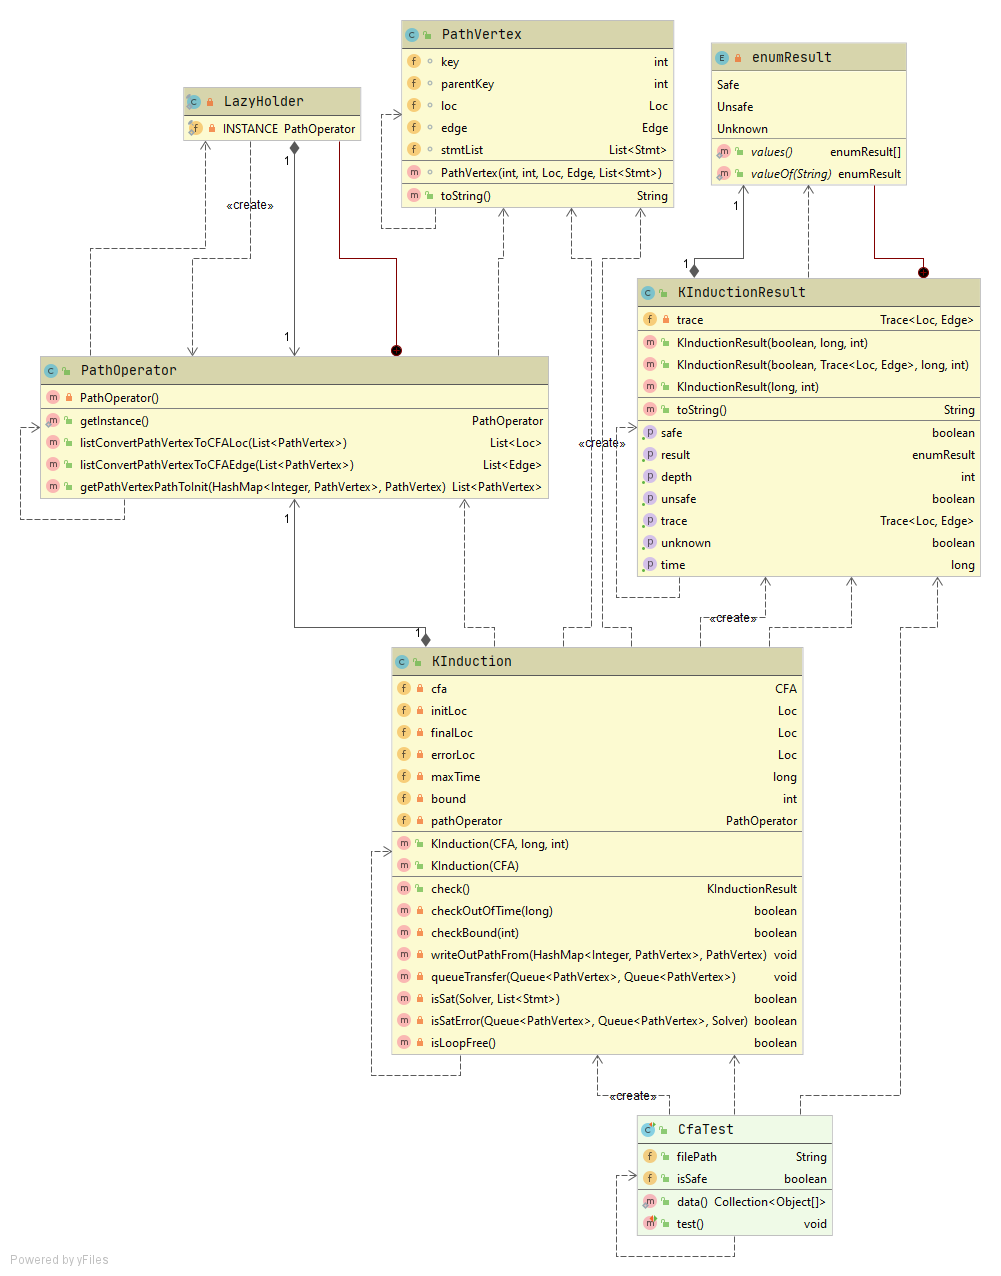
\includegraphics[width=150mm, keepaspectratio]{figures/allapot_diagram.png}
	\caption[Caption for LOF]{A programom UML állapotdiagramja.\textsuperscript{*}}
	\small\textsuperscript{*} Automatikusan generálva az IntelliJ Idea fejlesztőkörnyezettel
	\label{fig:state_diagram}
\end{figure}
\clearpage % TODO

\paragraph{Függvények.}
Miután van egy széles, de nem túl mély rálátásunk a programra, most elmerülnék benne és bemutatnám részletesebben, függvényekre bontva az osztályokat.
\begin{itemize}
	\item \textbf{\texttt{KInduction}} osztály
	\begin{itemize}
		\item \textcolor{blue}{KInduction(CFA cfa)} -- Az osztály egy paraméterű konstruktora.
		\begin{itemize}
			\item \textbf{Bemenet}: CFA modell
			\item \textbf{Kimenet}: -
		\end{itemize}
	
		\item \textcolor{blue}{KInduction(CFA cfa, long maxTime, int bound)} -- Az osztály három paraméterű konstruktora.
		\begin{itemize}
			\item \textbf{Bemenet}: CFA modell, maximális megengedett idő és maximális bejárható mélység.
			\item \textbf{Kimenet}: -
		\end{itemize}
	
		\item \textcolor{blue}{check()} -- Az osztály modellellenőrzést végző függvénye.
		\begin{itemize}
			\item \textbf{Bemenet}: -
			\item \textbf{Kimenet}: A verifikáció eredménye, az ellenpélda, az eltelt idő és az elért mélység összecsomagolva egy \texttt{KInductionResult} típusú objektumba.
		\end{itemize}
	
		\item \textcolor{blue}{checkOutOfTime(long timeInSeconds)} -- Ellenőrzi, hogy ha van megadott időkorlát akkor azt nem-e léptük már át.
		\begin{itemize}
			\item \textbf{Bemenet}: A program indulása óta eltelt idő másodpercben.
			\item \textbf{Kimenet}: Boolean.
		\end{itemize}
	
	
		\item \textcolor{blue}{checkBound(int depth)} -- Ellenőrzi, hogy ha van megadott mélységkorlát akkor azt nem-e léptük már át.
		\begin{itemize}
			\item \textbf{Bemenet}: Az aktuális bejárásra váró mélység.
			\item \textbf{Kimenet}: Boolean.
		\end{itemize}
	
		\item \textcolor{blue}{queueTransfer(Queue<PathState> copyFrom, Queue<PathState> pasteTo)} -- A korlátos szélességi kereséshez két sort használok, az egyik a még bejárandó helyeket tartalmazza, a másik az ebben a mélységben már bejárt helyeket tárolja. A mélység bejárása után az utóbbit (copyFrom) beleteszem a másikba (pasteTo), így haladva egyre beljebb a térben.
		\begin{itemize}
			\item \textbf{Bemenet}: Két, PathState állapotokat tartalmazó sor.
			\item \textbf{Kimenet}: A pasteTo sor tartalmazni fogja a copyFrom sor tartalmát (mást nem, mert előtte kiürítjük), a copyFrom sor pedig üres lesz.
		\end{itemize}
	
		\item \textcolor{blue}{isSat(Solver solver, List<Stmt> stmtList)} -- Megnézi a solver megoldó segítségével, hogy az utasításlistát tartalmazó stmtList kielégíthető-e.
		\begin{itemize}
			\item \textbf{Bemenet}: Egy Z3 megoldó és egy utasításlista.
			\item \textbf{Kimenet}: Boolean: ha kielégíthető, akkor igaz, különben hamis.
		\end{itemize}
	
		\item \textcolor{blue}{isErrorLocReachable(Queue<PathState> queueBW, Queue<PathState> queue2BW, Solver solver)} -- A hibahelyről hátrafelé indulva járja be a teret két, az előbb említetthez hasonló sorral. Minden meghíváskor egy mélységet halad, a solver megoldót az elérhető helyek ellenőrzéséhez használja.
		\begin{itemize}
			\item \textbf{Bemenet}: Két, PathState állapotokat tartalmazó sor és egy Z3 megoldó.
			\item \textbf{Kimenet}: Boolean: ha belátja, hogy a hibahely nem elérhető, akkor igaz, különben hamis.
		\end{itemize}
	\end{itemize}

	\item \textbf{\texttt{KInductionResult}} osztály
	\begin{itemize}
		\item \textcolor{blue}{KInductionResult(long time, int depth)} -- Az osztály két paraméteres konstruktora. Helyes használat esetén a \texttt{KIduction} osztály akkor inicializál ezzel egy objektumot, mikor a futás eredménye \textit{ismeretlen} volt.
		\begin{itemize}
			\item \textbf{Bemenet}: A program futási ideje illetve a mélység ameddig jutott.
			\item \textbf{Kimenet}: -
		\end{itemize}
	
		\item \textcolor{blue}{KInductionResult(boolean isSafe, long time, int depth)} -- Az osztály három paraméteres konstruktora. Helyes használat esetén a \texttt{KIduction} osztály akkor inicializál ezzel egy objektumot, mikor a futás eredménye \textit{helyes} volt.
		\begin{itemize}
			\item \textbf{Bemenet}: A program futási eredménye (hiba, ha nem \texttt{true} az érték), a program futási ideje illetve a mélység ameddig jutott.
			\item \textbf{Kimenet}: -
		\end{itemize}
	
		\item \textcolor{blue}{KInductionResult(boolean isUnsafe, Trace<CFA.Loc, CFA.Edge> trace, long time, int depth)} -- Az osztály négy paraméteres konstruktora. Helyes használat esetén a \texttt{KIduction} osztály akkor inicializál ezzel egy objektumot, mikor a futás eredménye \textit{nem helyes} volt. A Trace egy Theta beépített osztály, amelyben én az ellenpéldát tárolom.
		\begin{itemize}
			\item \textbf{Bemenet}: A program futási eredménye (hiba, ha nem \texttt{true} az érték), egy Trace típusú ellenpélda, a program futási ideje illetve a mélység ameddig jutott.
			\item \textbf{Kimenet}: -
		\end{itemize}
		\ \\
		Az osztály minden változója privát, ezért mindhez létezik \texttt{get} függvény. Ezeket külön nem sorolom fel.
	\end{itemize}

	\item \textbf{\texttt{PathOperator}} Singleton osztály
	\begin{itemize}
		\item \textcolor{blue}{getInstance()}
		\begin{itemize}
			\item \textbf{Bemenet}: -
			\item \textbf{Kimenet}: Az egyetlen static final PathOperator példány.
		\end{itemize}
	
		\item \textcolor{blue}{listConvertPathVertexToCFALoc(List<PathState> path)}
		\begin{itemize}
			\item \textbf{Bemenet}: PathState állapotokat tartalmazó lista.
			\item \textbf{Kimenet}: A PathState állapot helyei listában, ugyanabban a sorrendben.
		\end{itemize}
	
		\item \textcolor{blue}{listConvertPathVertexToCFAEdge(List<PathState> path)}
		\begin{itemize}
			\item \textbf{Bemenet}: PathState állapotokat tartalmazó lista.
			\item \textbf{Kimenet}: A PathState állapot élei listában, ugyanabban a sorrendben. A path lista utolsó PathState állapotának élét nem adja hozzá a listához, mert az a kezdőállapot éle lenne, ami pedig nincs (\texttt{null}).
		\end{itemize}
	
		\item \textcolor{blue}{getPathVertexPathToInit(HashMap<Integer, PathState> pathMap, PathState item)}
		\begin{itemize}
			\item \textbf{Bemenet}: PathState állapotokat és az egyedi kulcsukat tartalmazó HashMap és egy PathState állapot.
			\item \textbf{Kimenet}: Egy PathState lista (útvonal) az item PathState állapotból indulva, mely a HashMap kiinduló eleméig tart (ami vagy a kezdőhely vagy a hibahely).
		\end{itemize}
	\end{itemize}

	\item \textbf{\texttt{PathState}} osztály
	\begin{itemize}
		\item \textcolor{blue}{PathState(int key, int parentKey, CFA.Loc loc, CFA.Edge edge, List<Stmt> stmtList)} -- az osztály öt elemű konstruktora.
		\begin{itemize}
			\item \textbf{Bemenet}: A PathState egyedi kulcsa, melynek segítségével a HashMap-ben lehetséges keresni, a megelőző állapot kulcsa, az állapothoz rendelt hely, az él amin keresztül a helyhez értünk és egy Stmt lista, mely tárolja a kiindulási helytől a PathState helyéig vezető út állításait. 
			\item \textbf{Kimenet}: -
		\end{itemize}
	\end{itemize}

	\item \textbf{\texttt{KInductionCommandLine}} osztály
	\begin{itemize}
		\item \textcolor{blue}{main(final String[] args)} -- Létrehoz egy \texttt{KInductionCommandLine} objektumot aminek átadja a parancssori argumentumokat és aminek meghívja utána a \texttt{run()} függvényét.
		\begin{itemize}
			\item \textbf{Bemenet}: - Parancssori argumentumok.
			\item \textbf{Bemenet}: -
		\end{itemize}
		
		\item \textcolor{blue}{KInductionCommandLine(final String[] args)} -- A kapott parancssori argumentumokat eltárolja.
		\begin{itemize}
			\item \textbf{Bemenet}: - Parancssori argumentumok.
			\item \textbf{Bemenet}: -
		\end{itemize}
		
		\item \textcolor{blue}{run()} -- A parancssorból beolvasott paramétereket feldolgozza.
		\begin{itemize}
			\item \textbf{Bemenet}: -
			\item \textbf{Bemenet}: -
		\end{itemize}
	\end{itemize}

	\item \textbf{\texttt{CfaTest}} osztály
	\begin{itemize}
		\item \textcolor{blue}{test()} -- @Test annotációval ellátott függvény, mely a JUnit tesztelésért felelős.
		\begin{itemize}
			\item \textbf{Bemenet}: -
			\item \textbf{Bemenet}: -
		\end{itemize}
	\end{itemize}
\end{itemize}

\subsection{Működés}
Ebben az alfejezetben részletesen kifejtem a programom működésének folyamatát, melyet vázlatosan összefoglal a (\ref{fig:state_diagram2}) diagram.

\begin{enumerate}
	\item lépés: A program bemenetként kap egy CFA modellt és opcionálisan korlátozó feltételeket.
	\item lépés: A következő változókat inicializálja:
	\begin{enumerate}
		\item \texttt{depth} -- az aktuális, bejárásra váró mélységet tárolja, kezdetben nulla,
		\item \texttt{queue} -- tárolja az aktuális bejárandó mélység állapotait, kezdetben csak a kezdőállapotot tárolja,
		\item \texttt{queueTemp} -- az aktuális mélység bejárása közben talált elérhető állapotokat tárolja,
		\item \texttt{availablePaths} -- a bejárás utáni queueTemp méretét tárolja, a programkód jobb olvashatóságának érdekében van külön is vezetve,
		\item \texttt{queueBW} -- ugyanaz, mint a queue, csak a hátrafelé haladó kereséshez (\textit{BackWard}), kezdetben csak a hibaállapotot tárolja,
		\item \texttt{queueTempBW} -- ugyanaz, mint a queueTemp, csak a hátrafelé haladó kereséshez (\textit{BackWard}),
		\item \texttt{pathMap} -- egy HashMap mely PathState állapotokat tárol s azok egyedi kulcsait használja kulcsnak, kezdetben csak a kezdőállapotot tárolja, illetve
		\item a program futási idejének a mérését segítő változókat.
	\end{enumerate}
	\item lépés: Elindít egy végtelen ciklust.
	\item lépés: Növeli a \texttt{depth} változó értékét és beállítja a \texttt{availablePaths} értékét nullára.
	\item lépés: Ellenőrzi, hogy vannak -e korlátozások, és ha igen, teljesülnek-e:
	\begin{enumerate}
		\item Ha teljesülnek, létrehoz egy KInductionResult objektumot és befejezi a program a futását \textit{ismeretlen} válasszal,
		\item Ha nem teljesül egyik sem (vagy nincsenek), akkor megyünk tovább a következő lépésre.
	\end{enumerate}
	\item lépés: Végig iterál a \texttt{queue} vermen, és kiveszi belőle az éppen utolsó elemet (\texttt{item : PathState}).
	\begin{enumerate}
		\item Végig iterál az \texttt{item} állapot \texttt{loc} változójának a kimenő élein (\texttt{edge : CFA.Edge})
		\begin{enumerate}
			\item Eltárolja a \texttt{loc : CFA.Loc} helyet, ahova jutott az élen keresztül
			\item Az \texttt{item stmtList} listájának a végére beszúrja az \texttt{edge stmt} utasításait.
			\item Létrehoz egy új állapotot \texttt{nextPS : PathState} néven, melynek megad egy egyedi kulcsot, a szülő kulcsa az \texttt{item} egyedi kulcsa lesz, a helye a \texttt{loc} és az éle pedig az \texttt{edge}.
			\item \texttt{pathMap} HashMap-hez hozzáadja a \texttt{nextPS} állapotot.
			\item Ellenőrzi solver segítségével, hogy az \texttt{stmtList} kielégíthető-e.
			\begin{enumerate}
				\item Ha igen, \texttt{queueTemp} veremhez hozzáadja a \texttt{nextPS} változót, és megnöveli eggyel az \texttt{availablePaths} értékét.
			\end{enumerate}
		\end{enumerate}
	\end{enumerate}
	\item lépés: Beleteszi az üres \texttt{queue} verembe a \texttt{queueTemp} verem tartalmát. Utóbbit utána kiüríti.
	\item Ellenőrzi, hogy az \texttt{availablePaths} értéke nulla -e:
	\begin{enumerate}
		\item Ha nulla, létrehoz egy KInductionResult objektumot és befejezi a program a futását \textit{helyes} válasszal.
	\end{enumerate}
	\item Ellenőrzi, hogy a hibahely elérhető-e hátra felől:
	\begin{enumerate}
		\item Ugyanaz, mint a 6. lépés, csak \texttt{queue} helyett \texttt{queueBW} veremmel, \texttt{queueTemp} helyett \texttt{queueTempBW} veremmel, illetve egy lokális \texttt{availablePaths} változóval, leszámítva a \texttt{(a) $ \rightarrow $ iv} lépést: \texttt{pathMap} HashMap-hez itt nem adjuk hozzá a \texttt{nextPV} állapotot, mert az csak az ellenpélda meghatározásához kell, amit meg úgy értelmeztünk, hogy csak a kezdőhelyből indulhat ki.
		\item Ha \texttt{availablePaths} nem nulla, azaz van elérhető hely, akkor a modellről nem tudtunk meg új információt, csak továbbra is azt látjuk, hogy talán elérhető a hibahely. Ha viszont \texttt{availablePaths} nulla, azaz a hibahelytől bejárva a gráfot arra jutunk egy bizonyos szint után, hogy nincs több elérhető hely, azzal akkor beláttuk, hogy a hibahely nem érhető el.
		\item Ha a hibahely nem érhető el, akkor létrehoz egy KInductionResult objektumot és befejezi a program a futását \textit{helyes} válasszal.
	\end{enumerate}
	\item Ellenőrzi, hogy azok a helyek között, melyeket a most bejárt mélység után kaptunk (tehát amiket \texttt{queue} tárol), ott van-e a hibahely:
	\begin{enumerate}
		\item Végig iterál a \texttt{queue} vermen, az aktuális elem az \texttt{item : PathState}.
		\begin{enumerate}
			\item Ha az \texttt{item loc} helye a hibahely és elérhető (az \texttt{item stmtList} listáját a solver ki tudja elégíteni), akkor létrehoz egy KInductionResult objektumot és befejezi a program a futását \textit{nem helyes} válasszal.
		\end{enumerate}
	\end{enumerate}
	\item Ha ideáig eljutott a program, akkor a 4) lépésre ugrik, ezzel újra kezdve még egy szint bejárását.
\end{enumerate}

\begin{figure}[!ht]
	\centering
	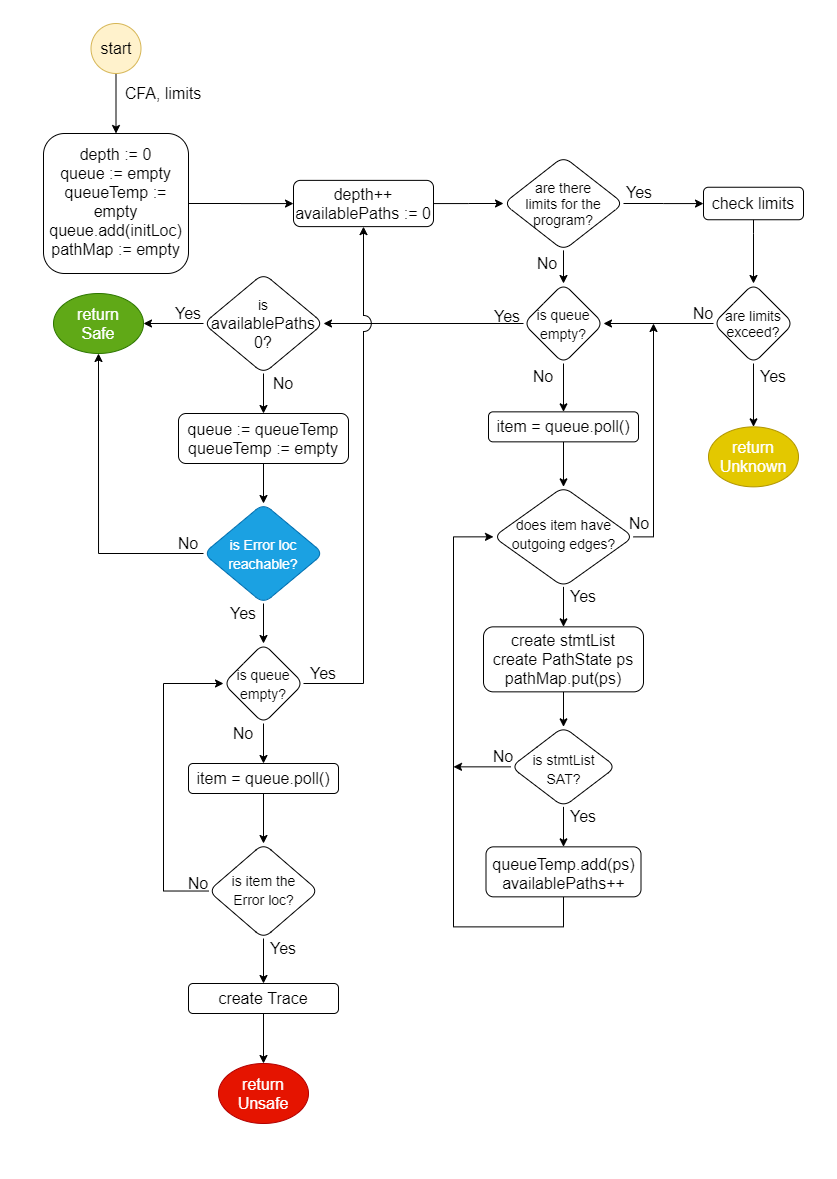
\includegraphics[width=150mm, keepaspectratio]{figures/flow_chart_med_res.png}
	\caption[Caption for LOF]{A programom folyamatábra diagramja.}
	\label{fig:state_diagram2}
\end{figure}
\clearpage

\subsection{Kimenet}
A program kimenetele egy \verb+KInductionResult+ osztályú objektum, melynek a következő változói vannak:

\begin{itemize}
	\item \verb+enumResult+ mely egy enum típusú változó és tárolja a program futásának a kimenetelét, ami az egyik a következőkből:
	\begin{itemize}
		\item Safe (\emph{Biztonságos})
		\item Unsafe (\emph{Nem biztonságos})
		\item Unknown (\emph{Ismeretlen})
	\end{itemize}
	\item \verb+trace+ mely egy \verb+Trace+ típusú változó és ami tárolja az ellenpéldát, ha van, különben \verb+null+.
	\item \verb+time+ mely \verb+long+ típusú és tárolja, hogy a program mennyi másodpercig futott.
	\item \verb+depth+ mely \verb+int+ típusú és azt mondja meg, hogy milyen mélységben fejeződött be a program futása.
\end{itemize}

A \textit{biztonságosról} és a \textit{nem biztonságosról} az előző fejezetekben sok szó esett. Az \textit{ismeretlen} válasszal a programom akkor tér vissza, ha kifutott az időből illetve ha elérte a maximális mélységet (a két feltétel között diszjunkció van), és addigra nem sikerült belátnia sem a modell helyességét, sem annak ellentettjét.